%----------------------------------------------------------------------
% Problem 2

\begingroup
\allowdisplaybreaks

\newpage
\section*{Problem 2}

\begin{figure}[h]
	\centering
	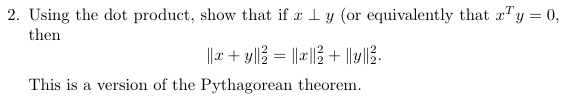
\includegraphics[width=0.8\textwidth]{./images/prob2_statement.png}
\end{figure}

\subsection*{Solution}

Consider column vectors of equal dimension $\bv{x},\,\bv{y} \in \R^{n}$. Let $\bv{x} \perp \bv{y}$, meaning that $\bv{x}^T \bv{y} = 0$. Also, recall that the dot product operator is \textit{additive} and \textit{distributive}.

\begin{align*}
	\twonorm{\bv{x} + \bv{y}}^2 &= \twonorm{\left(\bv{x} + \bv{y}\right)^T \left(\bv{x} + \bv{y}\right)} \\
	\\
	&= \twonorm{\bv{x}^T\bv{x}} + \twonorm{\bv{x}^T\bv{y}} + \twonorm{\bv{y}^T\bv{x}} + \twonorm{\bv{y}^T\bv{y}} \\
	\\
	&= \twonorm{\bv{x}^T\bv{x}} + \twonorm{\bv{x}^T\bv{y}} + \twonorm{\left(\bv{x}^T\bv{y}\right)^T} +\twonorm{\bv{y}^T\bv{y}} \\
	\\
	&= \twonorm{\bv{x}^T\bv{x}} + \cancelto{0}{\twonorm{\bv{x}^T\bv{y}}} + \cancelto{0}{\twonorm{\left(\bv{x}^T\bv{y}\right)^T}} + \twonorm{\bv{y}^T\bv{y}} \\
	\\
	&= \twonorm{\bv{x}^T\bv{x}} + \twonorm{\bv{y}^T\bv{y}} \\
	\\
	&= \twonorm{\bv{x}}^2 + \twonorm{\bv{y}}^2 \,\,\,\,\, \textcolor{green}{\checkmark}
\end{align*}



